\documentclass[12pt]{article}
\usepackage[left=2cm,right=2cm,top=2cm,bottom=2cm,letterpaper]{geometry}
\usepackage{lmodern}
\usepackage[T1]{fontenc}
\usepackage[utf8]{inputenc}
\usepackage[spanish,activeacute]{babel}
\usepackage{hyperref}
\usepackage{graphicx}
\graphicspath{{graphic/}}
\usepackage{float}
\usepackage{caption}
\usepackage[toc]{multitoc}
\setcounter{tocdepth}{2}
% automata
\usepackage{tikz}
\title{Proyecto 2}
\author{Carlos Gerardo Acosta Hernández \\ Andrea Itzel González Vargas \\ Luis Pablo Mayo Vega}
\date{Redes de Computadoras\\Facultad de Ciencias, UNAM}
%\setlength{\parindent}{0em}
\begin{document}
\maketitle
\tableofcontents
\newpage
\section{Especificación de requerimientos}
\subsection{Enunciado del problema}
De acuerdo con el modelo TCP/IP, \textit{la Capa de Aplicación} es la de mayor importancia y en la que se sustenta todo el desarrollo de redes de computadoras pues está compuesta por los protocolos y demás servicios encargados de manejar, intercambiar o decodificar los datos que los usuarios se envían a través de distintos hosts para comunicarse. En otras palabras, se busca que dos o más procesos en distintas computadoras puedan ser capaces de intercambiar información y de esta manera otorgar una mayor capacidad de procesamiento y mejor rendimiento del que se tendría con un único host.\\

Sin embargo, la \textit{Capa de Aplicación} no puede trabajar sola, siendo mediante un proceso de encapsulación en cada una de las capas, que los datos(PDU) se envian a las capas inferiores, añadiendo cada una de las capas información que le concierne para que sus protocolos puedan manejarlos.\\

Como sabemos, protocolos como \textsf{HTTP, DNS, FTP, SMTP o DHCP} tienen cada uno una estructura distinta ya bien definida y estandarizada en los articulos de \textit{Request for Comments} publicados, pero eso no significa que sean los únicos protocolos disponibles en la \textit{Capa de Aplicación}. La gran ventaja de esta capa es su adaptabilidad para que se desarrollen protocolos de acuerdo a las necesidades de la aplicación sobre la que se usarán. 

\subsection{Objetivo de la aplicación}

Esta aplicación fue creada con el objetivo de implementar un protocolo de la capa de aplicación en el que el usuario, conectado del lado del cliente, solicite un pokémon a capturar. El servidor elegirá aleatoriamente alguno de los pokémon que estén en su base de datos, se lo ofrecerá al usuario y, si éste acepta capturarlo, también aleatoriamente se indicará
 si logró capturarlo o no. \\

 El usuario también podrá ser capaz de consultar su Pokédex, con los nombres de los pokémon que ha capturado y la imagen de cada pokémon que seleccione. \\

 El protocolo que hemos diseñado se enfocará en las acciones del usuario y el servidor que involucren una comunicación entre ambos, cada una con un tipo de mensaje específico. Es decir, si un usuario quisiera capturar un pokémon, solo tendría que  enviar un mensaje con el código que el servidor entienda como "quiero capturar un pokémon" sin considerar otros aspectos como el nombre del pokémon o el tamaño de la imagen que contiene a tal pokémon. \\

 En ese sentido, diseñar nuestro propio protocolo nos permite tener mayor control sobre la tasa de transferencia de los datos dentro de la aplicación, disminuyendo los costos de la comunicación y mejorando el desempeño del programa.

 \newpage
 \subsubsection{Casos de uso}
 \begin{center}
   \begin{tabular}{|l|p{5cm}|p{9cm}|}
     \hline
     Actor & Caso de uso & Descripción \\
     \hline
     Pokentrenador & Iniciar sesión & El usuario se conecta con el servidor y se le muestra el menú principal de la aplicación \\ \hline
     Pokentrenador & Capturar pokémon & El usuario solicita al servidor que le muestre un pokémon y decide si intenta capturarlo (con un número finito de intentos) o no\\ \hline
     Pokentrenador & Consultar pokedex & El usuario hace una consulta para buscar un pokémon en su pokédex \\ \hline
     Pokentrenador & Cerrar sesión & Cierra la conexión con el servidor \\
     \hline
   \end{tabular}
 \end{center}
 \begin{figure}[H]
   \centering
   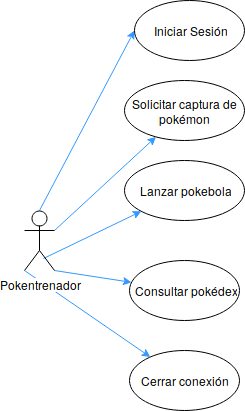
\includegraphics[width=0.4\textwidth]{casosdeuso}
   \caption{Diagrama de casos de uso de la aplicación}
 \end{figure}
 
\section{Diseño del protocolo}
\subsection{Máquina de Estados Finita}
Máquina de Estados Finita para el protocolo de la capa de aplicación.
\begin{center}
\begin{tikzpicture}[scale=0.2]
\tikzstyle{every node}+=[inner sep=0pt]
\draw [black] (7.7,-22) circle (3);
\draw (7.7,-22) node {$q_0$};
\draw [black] (21.9,-21.4) circle (3);
\draw (21.9,-21.4) node {$q_1$};
\draw [black] (35.4,-21.4) circle (3);
\draw (35.4,-21.4) node {$q_2$};
\draw [black] (63.3,-21.4) circle (3);
\draw (63.3,-21.4) node {$q_3$};
\draw [black] (35.4,-7.3) circle (3);
\draw (35.4,-7.3) node {$q_4$};
\draw [black] (63.3,-46.6) circle (3);
\draw (63.3,-46.6) node {$q_5$};
\draw [black] (35.4,-46.6) circle (3);
\draw (35.4,-46.6) node {$q_6$};
\draw [black] (7.7,-49.9) circle (3);
\draw (7.7,-49.9) node {$q_9$};
\draw [black] (9.968,-20.054) arc (121.77715:63.06187:9.706);
\fill [black] (19.48,-19.65) -- (18.99,-18.84) -- (18.54,-19.74);
\draw (14.59,-18.02) node [above] {$c:10$};
\draw [black] (24.9,-21.4) -- (32.4,-21.4);
\fill [black] (32.4,-21.4) -- (31.6,-20.9) -- (31.6,-21.9);
\draw (28.65,-21.9) node [below] {$s:20$};
\draw [black] (19.52,-23.209) arc (-61.01633:-114.14465:10.403);
\fill [black] (10.22,-23.6) -- (10.75,-24.39) -- (11.16,-23.47);
\draw (15,-25.09) node [below] {$s:44$};
\draw [black] (34.348,-24.204) arc (-26.53097:-150.98729:14.4);
\fill [black] (8.87,-24.76) -- (8.82,-25.7) -- (9.7,-25.21);
\draw (21.8,-32.71) node [below] {$c:11$};
\draw [black] (37.033,-9.805) arc (25.08093:-25.08093:10.722);
\fill [black] (37.03,-9.81) -- (36.92,-10.74) -- (37.82,-10.32);
\draw (38.54,-14.35) node [right] {$c:12$};
\draw [black] (34.029,-18.74) arc (-159.56755:-200.43245:12.574);
\fill [black] (34.03,-18.74) -- (34.22,-17.82) -- (33.28,-18.16);
\draw (32.74,-14.35) node [left] {$s:21/e:44$};
\draw [black] (38.4,-21.4) -- (60.3,-21.4);
\fill [black] (60.3,-21.4) -- (59.5,-20.9) -- (59.5,-21.9);
\draw (49.35,-21.9) node [below] {$c:13$};
\draw [black] (63.3,-24.4) -- (63.3,-43.6);
\fill [black] (63.3,-43.6) -- (63.8,-42.8) -- (62.8,-42.8);
\draw (62.8,-34) node [left] {$s:22$};
\draw [black] (38.199,-45.523) arc (108.58634:71.41366:34.985);
\fill [black] (38.2,-45.52) -- (39.12,-45.74) -- (38.8,-44.79);
\draw (49.35,-43.2) node [above] {$c:15$};
\draw [black] (60.488,-47.642) arc (-72.05358:-107.94642:36.146);
\fill [black] (60.49,-47.64) -- (59.57,-47.41) -- (59.88,-48.36);
\draw (49.35,-49.9) node [below] {$s:23$};
\draw [black] (35.4,-43.6) -- (35.4,-24.4);
\fill [black] (35.4,-24.4) -- (34.9,-25.2) -- (35.9,-25.2);
\draw (35.9,-34) node [right] {$s:24/e:41$};
\draw [black] (7.7,-25) -- (7.7,-46.9);
\fill [black] (7.7,-46.9) -- (8.2,-46.1) -- (7.2,-46.1);
\draw (7.2,-35.95) node [left] {$c:00$};
\draw [black] (61.07,-44.59) -- (37.63,-23.41);
\fill [black] (37.63,-23.41) -- (37.88,-24.32) -- (38.56,-23.58);
\draw (51.59,-33.51) node [above] {$c:14$};
\end{tikzpicture}
\end{center}


\subsection{Descripción de los estados}
\begin{center}
\begin{tabular}{|l|p{9cm}|}
  \hline
  Estado & Descripción \\
  \hline
  $q_0$ & Conexión establecida, inicio de aplicación. \\ \hline
  $q_1$ & Inicio de sesión. \\ \hline
  $q_2$ & Menú de juego. \\ \hline
  $q_3$ & Solicitud de captura de \textit{pókemon}. \\ \hline
  $q_4$ & Búsqueda de un pókemon en la \textit{pókedex}. \\ \hline
  $q_5$ & Aparición de un \textit{Pókemon} salvaje. \\ \hline
  $q_6$ & Intento de captura de \textit{pókemon}.\\ \hline
  $q_9$ & Cierre de conexión. \\
  \hline
\end{tabular}
\end{center}
\newpage

\subsection{Descripción de los mensajes en la comunicación cliente-servidor}
\begin{center}
  \begin{tabular}{|l|c|p{5.9cm}|}
    \hline
    Código & Segmento & Descripción \\ \hline
    \hline
    00 & \texttt{|long|code|} & Termina la conexión para un cliente. \\ \hline
    10 & \texttt{|long|code|name|} & Solicitud de inicio de sesión del cliente. El parámetro \texttt{name} se refiere al nombre de usuario del cliente. \\ \hline
    11 & \texttt{|long|code|} & Solicitud de cierre de sesión del cliente. \\ \hline
    12 & \texttt{|long|code|name|} & Acceso y consulta a la \textit{Pokédex} mediante el nombre de un pokémon. \\ \hline
    13 & \texttt{|long|code|} & Acceso a la opción de captura. \\ \hline
    14 & \texttt{|long|code|} & El usuario rechaza el pokémon salvaje ofrecido por el servidor. \\ \hline
    15 & \texttt{|long|code|attempts|name|} & Intento de captura del pokémon salvaje ofrecido. \\ \hline %%dfdishffjsjfsfvkfdjhJNDSJFNSDGLDKN
    \hline
    20 & \texttt{|long|code|} & Inicio de sesión del cliente exitoso. \\ \hline
    21 & \texttt{|long|code|long\_n|name|long\_img|img} & Resultado exitoso de la Pokédex con imagen del pokémon. \\ \hline %wat
    22 & \texttt{|long|code|attempts|name|} & Selección aleatoria de un pokémon salvaje para el cliente. Incluye el máximo número de intentos. \\ \hline
    23 & \texttt{|long|code|attempts|name|} & Pokémon no capturado, disminución del número de intentos. \\ \hline
    24 & \texttt{|long|code|long\_n|name|long\_img|img|} & Pokémon capturado con imagen incluída. \\ \hline \hline
    41 & \texttt{|long|code|} & Error: Máximo número de intentos de captura alcanzados. \\ \hline
    44 & \texttt{|long|code|} & Error: Consulta infructuosa. \\ \hline
  \end{tabular}
\end{center}

\subsection{Diseño de la base de datos}
 \begin{figure}[H]
   \centering
   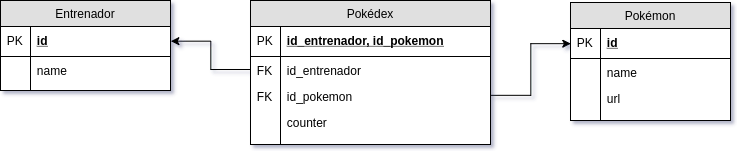
\includegraphics[width=1\textwidth]{PokeDB2}
   \caption{Diagrama de casos de uso de la aplicación}
 \end{figure}
\section{Implementación del protocolo}
\subsection{Especificación del ambiente de desarrollo}
%revisar versiones
\begin{tabular}{l r l r}
  \textbf{Lenguaje de programación:} & Java & \textbf{versión:} & 1.8 \\
  \textbf{Herramienta de construcción de software:} & Apache Ant & \textbf{versión:} & 1.9.9 \\
  \textbf{Sistema Manejador de Base de Datos:} & sqlite & \textbf{versión:} & 2.8.17 \\
  \textbf{Driver de conectividad JDBC:} & sqlite-jdbc & \textbf{versión:}3,16,1\\
  \textbf{Pruebas Unitarias:} & JUnit & Hamcrest \\
\end{tabular}

\newpage
\subsection{Estructura del proyecto}  
\begin{verbatim}
.
|- proyecto2.jar
|- build
|- - ConexionBD.class
|- - redes
|- - - MultiThreadPrueba.class
|- - - Mensaje12.class
|- - - Mensaje21.class
|- - - ConexionBD.class
|- - - Mensaje24.class
|- - - Estado.class
|- - - ClienteHilo.class
|- - - FabricaMensaje.class
|- - - MensajeGenerico.class
|- - - Pokentrenador$1.class
|- - - Mensaje15.class
|- - - Pokentrenador.class
|- - - Controlador.class
|- - - test
|- - - - ControladorTest.class
|- - - Mensaje10.class
|- - - Pokeservidor.class
|- - - Mensaje22.class
|- - - Proyecto2.class
|- - - MultiThreadPrueba$Hilo.class
|- - - Imagen.class
|- - - Mensaje23.class
|- - - ClienteHilo$1.class
|- static
|- - requirements
|- - poke_script.py
|- man
|- - proyecto2.1
|- - proyecto2.1.gz
|- documentos
|- - proyecto2.out
|- - proyecto2.log
|- - graphic
- - - 
- - proyecto2.toc
- - proyecto2.tex
- - proyecto2.pdf
- - proyecto2.aux
- doc
- - proyecto2.out
- - proyecto2.log
- - proyecto2.toc
- - proyecto2.pdf
- - proyecto2.aux
- src
- - sql
- - - poke_app_db.sql
- - redes
- - - Mensaje10.java
- - - Estado.java
- - - MultiThreadPrueba.java
- - - Pokeservidor.java
- - - MensajeGenerico.java
- - - Mensaje15.java
- - - Imagen.java
- - - Controlador.java
- - - Pokentrenador.java
- - - ClienteHilo.java
- - - ConexionBD.java
- - - Mensaje24.java
- - - test
- - - - ControladorTest.java
- - - Mensaje22.java
- - - Mensaje21.java
- - - Mensaje23.java
- - - FabricaMensaje.java
- - - Mensaje12.java
- - - Proyecto2.java
- build.xml
- arbol.txt
- lib
- - junit.jar
- - hamcrest-core.jar
- - sqlite-jdbc-3.16.1.jar
\end{verbatim}

\section{Uso y pruebas del protocolo}
\subsection{Manual de uso}
\subsubsection{Instalación y conexión de cliente/servidor}
La aplicación cuenta con una página de manual para sistemas operativos *NIX, en donde se detalla más en el uso de la aplicación con algunos ejemplos sencillos. \\
Para poder compilar y ejecutar el programa por primera vez, se requiere contar con la versión 1.8 o superior de \texttt{Java} así como la versión 1.9.9 o superior de \texttt{Apache Ant}, entonces puede emplear el comando: \\
\begin{verbatim}
[user@host p02] ant 
\end{verbatim}
Y el sistema automatizado de \texttt{Apache Ant} generará todos los archivos necesarios para que el programa funcione. En caso de haber errores, el mismo \texttt{Ant} le indicará cuáles son. \\

Una vez compilado, se puede iniciar la aplicación con la instrucción en linea de comando:
\begin{verbatim}
[user@host p02] java -jar proyecto2 
\end{verbatim}

\subsubsection{Inicio de sesión}
Una vez establecida la conexión entre cliente y servidor, el servidor le pedirá al usuario que ingrese su nombre para poder iniciar sesión o cerrar la conexión entre ambos hosts. Si el nombre de usuario ingresado se encuentra registrado en la base de datos de la aplicación, el servidor le mostrará al usuario con sesión iniciada su menú principal de juego.

\subsubsection{Uso dentro de la aplicación}
Una vez iniciada la sesión del usuario, éste tendrá acceso a un menú principal en el que se muestre las opciones que le otorga la aplicación, como capturar un pokémon, consultar su pokédex o cerrar sesión. \\

Si el usuario quiere capturar un pokémon, el servidor le mostrará aleatoriamente alguno de los nombres de pokémon registrados y el usuario decidirá si desea o no capturarlo. Si acepta el desafío, tendrá que lograr capturarlo antes de llegar al límite de intentos permitido. \\

Para consultar su pokédex, el usuario deberá ingresar el nombre del pokémon que quiera buscar. Si el pokémon ya fue capturado, se le mostrará la imagen de tal pokémon y recibirá un mensaje de error si el nombre del pokémon no es el correcto o el usuario no lo ha capturado. \\

Si el usuario decide cerrar su sesión, regresará a la pantalla de inicio de la aplicación y se le preguntará si desea iniciar sesión de nuevo o cerrar la conexión entre los hosts. \\

\subsection{Demostración del funcionamiento}

\end{document}
